
Recommendation system is one of the most important tools for most websites. Various websites, recommend a variety of products to their users, for e.g. books, movies, songs, ads, etc. But these products can’t be separated, while there are products which can be separated into different parts and categories, like outfits. As online shopping and fashion-focused social networks are growing rapidly, there is a great need for intelligent fashion recommendation. Retailers have to spend a large amount of time to come up with different combinations of their products that would as a whole, go well as an outfit, and even then, the options aren’t really personalized. \newline

Hence, our project will have two main components, a web application and a recommendation system. Therefore, our literature review is divided into two parts.

\section{Web-Application}
The literature review for our web-application is divided into three domains. Technologies used for client-side, server-side and the API for establishing the interaction between them. \newline

 \autoref{table:tech-server}, \autoref{table:tech-client}, and \autoref{table:tech-api} offer a detailed comparison between different communication interfaces.
 
\begin{table}[H]
\begin{tabular}{ @{}|p{4cm}|p{3cm}|p{4cm}|p{3cm}|  }
 \hline
 \multicolumn{4}{|c|}{\textbf{Server-side Technologies}} \\
 \hline
 \textbf{Django} & \textbf{Tornado} & \textbf{ASP.NET} & \textbf{Node.JS}\\
 \hline
 In Python, good support for ML out of the box.   & Also In Python, good support for ML out of the box.    & In C\#, Visual Basic, F\#, high dependency on external ecosystems for ML, not as intuitive. & In JavaScript, moderate support for ML out of the box.\\
  \hline
 High community support.&   Low community support.  & Moderate community support. & High community support.\\
  \hline
Not completely asynchronous, though offers support. &  Highly synchronous. & Supports both, synchronous as well as asynchronous operations. & Supports both, synchronous as well as asynchronous operations. \\
  \hline
Supports direct integration with React/Front-end frameworks/AJAX & Third-party libraries for integration. & Completely different eco-system & Direct integration with React and Angular.\\
 \hline
 Offers abstraction, is high level. & Also high level.  & Relatively low-level. & Relatively low-level.\\
 \hline
\end{tabular}
\caption{Technology Comparison: Server-side Communication}
\label{table:tech-server}
\end{table}

\begin{table}[H]
\begin{tabular}{ @{}|p{5cm}|p{5cm}|p{5cm}|  }
 \hline
 \multicolumn{3}{|c|}{\textbf{Client-side Technologies}} \\
 \hline
 \textbf{Django} & \textbf{React} & \textbf{Angular} \\
 \hline
 Bound to a Django server, imposes design and flow restrictions.  & Not bound to a specific server, gives high design freedom.  & Not bound to a specific server, gives moderate design freedom.\\
  \hline
Complete framework, potential overheads. & Only a library on top of JS, low overheads.  & Complete framework, potential overheads.\\
 \hline
 Low community support. &  High community support. & Moderate community support. \\
  \hline
Offers high throughput in development. & Offers high throughput performance-wise. & Offers high throughput performance-wise.\\
 \hline
\end{tabular}
\caption{Technology Comparison: Client-side Communication}
\label{table:tech-client}
\end{table}

\begin{table}[H]
\begin{tabular}{ @{}|p{7cm}|p{7cm}|  }
 \hline
 \multicolumn{2}{|c|}{\textbf{API Technologies}} \\
 \hline
 \textbf{REST} & \textbf{GraphQL} \\
 \hline
 Every resource is identified by a unique URL having its own end-point that requires router handlers.  & Resources are identified by fields in their schema representation with individual resolvers.\\
 \hline
 Each request calls exactly one route handler, for a nested query, this leads to overheads. & Each query can call many resolvers to construct a nested response with multiple resources. \\ 
 \hline
 The response shape has to be manually constructed and is kept fixed. &  The response shape is constructed automatically to match the query shape.  \\
  \hline
 As a result, resource type, shape, \& fetch query are coupled.  & Everything is de-coupled leading to higher scalability.\\
 \hline
\end{tabular}
\caption{Technology Comparison: API-level Communication}
\label{table:tech-api}
\end{table}

\textbf{Our Approach}\\
Based on the project requirements and keeping the communication channels in mind, the chosen technology stack for the client-end is: TypeScript, React, and \href{https://github.com/apollographql/react-apollo}{React Apollo} (for interacting with the GraphQL API), and for the server-end is: Python, Django, and \href{https://github.com/graphql-python/graphene-django}{Graphene Django} (for creating the GraphQL API).

\section{Recommendation System}
This literature review regarding recommendation system, aims to compare the various methods and techniques studied in the existing work for recommendation systems. It is divided into two domains, the dataset and recommendation engine.

\subsection{Dataset}
The largest and best annotated publicly available dataset in the domain of fashion is \textbf{DeepFashion}.

The DeepFashion dataset consists of more than 800,000 richly annotated images, ranging from well-posed shop images to unconstrained consumer photos, making it twice the size of the largest previously available dataset. Each image in the dataset is labeled with 50 categories, 1,000 descriptive attributes, and clothing landmarks.

Another strength of the DeepFashion dataset is that it contains rigorous benchmark for testing the performance of algorithms for clothes recognition. The three benchmarks it contains are clothing attribute prediction, in-shop clothes retrieval, and cross-domain clothes retrieval, a.k.a. street-to-shop. All three are relevant for the scope 

\begin{enumerate}
	\item \textbf{Category and Attribute Annotation:} Each image is labelled with a single category label. There are a total of 50 mutually exclusive categories, labelled by human annotators. The dataset also contains 1000 attributes which are extracted from image metadata. However, these are not utilized by our model. There are 63,720 diverse images in this benchmark.
	
	\item \textbf{In-Shop Clothes Retrieval:} This task determines if two in-shop images belong to the same clothing item. This benchmark contains 54,632 images of 11,735 clothing items.  
	
	\item \textbf{Consumer-to-Shop Clothes Retrieval:} Aimed at matching consumer-taken photos with their shop counterparts. Contains 251,361 consumer-to-shop image pairs.
\end{enumerate}

\begin{figure}[H]
\includegraphics[width=15cm]{images/dataset-comparision.pdf} 
\centering
\caption{Dataset Comparison}
\label{dataset:home}
\end{figure}

%Tanseng et al. \cite{paperone} and Tong et al. \cite{papertwo} have used the Polyvore dataset, which consists of 409k outfits consisting of 644,192 images of items. It is created by users and has up to 8 items per image. Whereas, Ziwei et al. \cite{paper3} have used DeepFashion dataset. It is publicly available and consists of more than 800,000 images, labelled with 50 categories and 1000 descriptive tag (attributes), bounding boxes and other information. \newline
 
\textbf{Our Approach} \newline
We will be using DeepFashion dataset as it contains large number of outfit images which are vastly categorized and labelled to train our model and benchmark performance. We will then train the model further on our local dataset, scraped from local stores like, Export Leftovers, J. Furor, Zellbury, etc. As eastern data is comparatively less, our model would suffer from overfitting if used as the only source. 

\subsection{Recommendation Engine}


Viet et al. \cite{paper4} learned featured transformation for measuring compatibility between different pairs of items using a Siamese CNN architecture, whereas, McAuley et al. \cite{paper5} used parametric distance transformation for the same purpose. Parametric distance transformation assigns the lowest distance to pairs of clothing which fit well. However, these techniques only gave the matching pairs of clothing and didn’t take the personalization issue into account. The initial attempt to explore the personalized outfit recommendation was made by Hu et al. \cite{paperseven}, using functional tensor factorization method, however, they used hand-crafted features.  \newline

Recently, researchers have explored deep networks and have begun to apply deep learning to recommendation systems. \autoref{table:recommendation-engine 1}, \autoref{table:recommendation-engine 2}, and \autoref{table:recommendation-engine 3} gives a detailed comparison between different approaches used in multiple research papers. \newline

\begin{table}[H]
\begin{tabular}{ @{}|p{3cm}|p{4cm}|p{2.5cm}|p{2.5cm}|p{2.5cm}|  }
 \hline
 \multicolumn{5}{|c|}{\textbf{Recommendation Engine}} \\
 \hline
 \textbf{Research Paper} & \textbf{Approach} & \textbf{Dataset} & \textbf{Resources} & \textbf{Time}\\
 \hline
Large Scale Visual Recommendations From Street Fashion Images.
  & Recommends visually complementary items using Deterministic Fashion Recommenders (DFR) and Stochastic Fashion Recommender.
    & Fashion-136K, Fashion-350K, Fashion-Q1K datasets. & Not mentioned. & Not mentioned.\\
\hline
\end{tabular}
\caption{Technology Comparison: Recommendation Engine}
\label{table:recommendation-engine 1}
\end{table}


\begin{table}[H]
\begin{tabular}{ @{}|p{3cm}|p{4cm}|p{2.5cm}|p{2.5cm}|p{2.5cm}|  }
 \hline
 \multicolumn{5}{|c|}{\textbf{Recommendation Engine}} \\
 \hline
 \textbf{Research Paper} & \textbf{Approach} & \textbf{Dataset} & \textbf{Resources} & \textbf{Time}\\
 \hline
 
  Learning visual similarity for product design with convolutional neural networks. & 
Training with stochastic gradient descent. t-SNE algorithm to visualize the result. & Dataset made from Houzz.com. & MTurk to collect the necessary bounding boxes. AlexNet to detect both near and exact duplicates. & Using a Grid K520 GPU it took 100 ms to compute.\\
\hline

MatchNet: Unifying Feature and Metric Learning for Patch-Based Matching. & Deep convolutional network extracts features and a network of three FC layers computes similarity. Feature network is influenced by AlexNet. ReLU for the convolution layers. & UBC patch dataset. & AlexNet & 18 hours to 1 week to train the full network.\\
  \hline
FashionNet: Personalized Outfit Recommendation with Deep Neural Network. & VGGNet feature network for feature extraction and multi-layer fully connected network for computing clothes compatibility. & Dataset collected from Polyvore & VGGNet. Caffe. & Not mentioned. \\
 \hline
 
\end{tabular}
\caption{Technology Comparison: Recommendation Engine}
\label{table:recommendation-engine 2}
\end{table}

\begin{table}[H]
\begin{tabular}{ @{}|p{3cm}|p{4cm}|p{2.5cm}|p{2.5cm}|p{2.5cm}|  }
 \hline
 \multicolumn{5}{|c|}{\textbf{Recommendation Engine}} \\
 \hline
 \textbf{Research Paper} & \textbf{Approach} & \textbf{Dataset} & \textbf{Resources} & \textbf{Time}\\
 \hline
 DeepFashion: Powering Robust Clothes Recognition and Retrieval with Rich Annotations. & FashionNet simultaneously predicts landmarks and attributes. Network structure similar to VGG-16 except last convolutional layer, which is replaced by three branches of layers. Regression loss for landmark localization. Softmax loss for the predictions of categories. Triplet loss for metric learning & 800, 000 diverse
 fashion images ranging from well-posed shop images to unconstrained consumer photos. 
 Mogujie, Forever21 and Google Images & FashionNet to demonstrate usefulness. & Not mentioned. \\
\hline

Using Very Deep Autoencoders for Content-Based Image Retrieval & Train RBM by standard contrastive divergence learning procedure. To reduce noise, we use the probabilities rather than the stochastic binary states. Fine Tune auto-encoder by back propogation.  & Preprocessed 1.6 million 32 × 32 color images. CIFAR-10 dataset. & Restricted Boltzmann Machines. & 2 days on Nvidia GTX 285 GPU \\
\hline

\end{tabular}
\caption{Technology Comparison: Recommendation Engine}
\label{table:recommendation-engine 3}
\end{table}


\textbf{Our Approach}
\newline

The paper "MatchNet: Unifying Feature and Metric Learning for Patch-Based Matching" \cite{matchnet}, published by Google Research in 2015 served as the inspiration for the FashionNet architecture proposed by the creators of DeepFashion. They use a single network to simultaneously predict both landmarks and attributes. The structure of this network is similar to VGG-16, with the last convolutional layer replaced by three branches of layers carefully designed for clothes.

\begin{figure}[H]
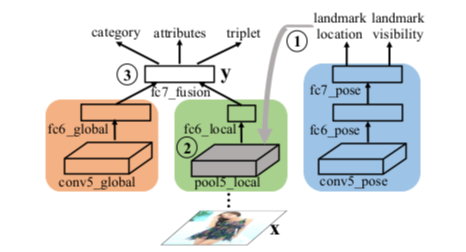
\includegraphics[width=10cm]{images/fashionnet-architecture.png} 
\centering
\caption{FashionNet Architecture \cite{deepfashion}}
\label{architecture}
\end{figure}

However, since the only task we wish to perform in this project is in-shop retrieval and in the interest of making our model simpler, we decided to use an approach relying on only a feature network and use Euclidean distance to find similar vectors. Our feature network will consist of a ResNet50 model trained on the DeepFashion clothing classification benchmark using transfer learning. This feature network will convert images into a 512-dim feature vector. We will then query the database to retrieve images who's feature vector has minimum euclidean distance from the query feature vector. 

%\cite{einstein} but wish the work was typeset in \LaTeX \cite{knuthwebsite}, e.g. by taking help from \cite{latexcompanion}.